\documentclass[compress]{beamer}
%\documentclass[compress, handout]{beamer}

% To create a handout: uncomment below and add handout as an option
% for documentclass
%\usepackage{pgfpages}
%\pgfpagesuselayout{2 on 1}[a4paper,border shrink=5mm]

\usepackage[T1]{fontenc}
\usepackage[ngerman]{babel}
\usepackage[utf8]{inputenc}
\usepackage{units}
\usepackage{amsmath}
\usepackage{amsfonts}
\usepackage[amssymb]{SIunits}
\usepackage{amssymb}
\usepackage{microtype}
\usepackage{bbm}
\usepackage{booktabs}
\usepackage{fancyvrb}
\usepackage{color}
\usepackage{pygments}
\usepackage{stackrel}
\usepackage{MnSymbol}

\usepackage[TOC]{style} % add option 'TOC' if you want an Outline before every section
\usepackage{simpleMath}

\usepackage{graphicx}
%\graphicspath{{Figures/}}


\title[] % (optional, use only with long paper titles)
{Python Programming for Scientists}
\titlegraphic{
\includegraphics[width=0.9\textwidth]{Figures/NAT_SIGN_druck_SW}\\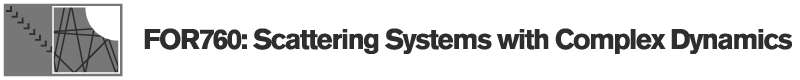
\includegraphics[width=0.9\textwidth]{Figures/FOR760_full}}
%\subtitle{A good subtitle} % (optional)
\author[] % (optional, use only with lots of authors)
{Alexander Eberspächer}

\date[]{October 12\textsuperscript{th} 2011} % \today ?

\subject{Python Programming for Scientists}


\begin{document}

\begin{frame} % title
  \titlepage
  \thispagestyle{empty}
\end{frame}

\begin{frame}{Outline} % first Outline
  \tableofcontents
\end{frame}

% Input your presentation's contents here
\section{Introduction}

\subsection{The setting}

% slide
\begin{frame}{Who uses...}

\begin{itemize}
	\item We all use computers to generate or process data
\end{itemize}

Question to the audience: who uses...

\begin{columns}[t]

\column{0.5\textwidth}

\begin{itemize}
	\item C/C++?
	\item Fortran?
	\item Ada?
	\item Java?
	\item Matlab/Octave?
\end{itemize}

\column{0.5\textwidth}

\begin{itemize}
	\item IDL?
	\item Perl?
	\item Ruby?
	\item \alert{Python}?
\end{itemize}

\end{columns}

\end{frame}

% Slide
\begin{frame}{What is Python?}

Python is/has...

\begin{columns}[t]

\column{0.5\textwidth}

\begin{itemize}
	\item a scripting language
	\item general purpose
	\item interpreted
	\item easy to learn
	\item clean syntax
\end{itemize}

\column{0.5\textwidth}

\begin{itemize}
	\item multi-paradigm
	\item open-source
	\item available for all major platforms
	\item great community
\end{itemize}

\end{columns}

\end{frame}

\subsection{The best of all}


\begin{frame}{The best of all:}

\begin{exbox}{Python comes...}
	... with \alert{batteries included}!
\end{exbox}

\vspace{-1.25ex}

\begin{center}
	Libraries available for...
\end{center}

\vspace{-4.5ex}

\begin{columns}[t]

\column{0.3\textwidth}

\begin{center}
	daily IT needs...
\end{center}

\vspace{-2.5ex}

\begin{itemize}
	\item networks
	\item OS interaction
	\item temporary files
	\item zip files
	\item ...
\end{itemize}

\column{0.7\textwidth}

\begin{center}
	\alert{science!}
\end{center}

\vspace{-2.5ex}

\begin{itemize}
	\item efficient array operations (\emph{NumPy})
	\item general numerical algorithms (\emph{SciPy})
	\item 2D visualization (\emph{matplotlib})
	\item 3D visualization (Mayavi)
	\item special problems (e.g. finite elements with FEniCS, quantum optics with QuTiP)
	\item symbolic math (SageMath, sympy)
	\item ...
\end{itemize}

\end{columns}

\end{frame}


\section{Basics}

\subsection{Hello, World!}

\begin{frame}[fragile]{Scientific \emph{Hello, World!}}

\begin{columns}

\column{0.65\textwidth}

\begin{Verbatim}[commandchars=\\\{\}]
\PY{k+kn}{import} \PY{n+nn}{sys}
\PY{k+kn}{from} \PY{n+nn}{math} \PY{k+kn}{import} \PY{n}{sin}\PY{p}{,} \PY{n}{pi}

\PY{k}{def} \PY{n+nf}{sincSquare}\PY{p}{(}\PY{n}{x}\PY{p}{)}\PY{p}{:}
    \PY{l+s+sd}{"""Return sinc(x)\PYZca{}2.}
\PY{l+s+sd}{    """}
    \PY{k}{if}\PY{p}{(}\PY{n}{x} \PY{o}{<}\PY{o}{>} \PY{l+m+mf}{0.0}\PY{p}{)}\PY{p}{:}
        \PY{k}{return} \PY{p}{(}\PY{n}{sin}\PY{p}{(}\PY{n}{pi}\PY{o}{*}\PY{n}{x}\PY{p}{)}\PY{o}{/}\PY{p}{(}\PY{n}{pi}\PY{o}{*}\PY{n}{x}\PY{p}{)}\PY{p}{)}\PY{o}{*}\PY{o}{*}\PY{l+m+mi}{2}
    \PY{k}{else}\PY{p}{:}
        \PY{k}{return} \PY{l+m+mf}{1.0}

\PY{n}{x} \PY{o}{=} \PY{n}{sys}\PY{o}{.}\PY{n}{argv}\PY{p}{[}\PY{l+m+mi}{1}\PY{p}{]}
\PY{n}{y} \PY{o}{=} \PY{n}{sincSquare}\PY{p}{(}\PY{n+nb}{float}\PY{p}{(}\PY{n}{x}\PY{p}{)}\PY{p}{)}
\PY{k}{print}\PY{p}{(}\PY{l+s}{"}\PY{l+s}{sinc(}\PY{l+s+si}{\PYZpc{}s}\PY{l+s}{)\PYZca{}2 = }\PY{l+s+si}{\PYZpc{}s}\PY{l+s}{"}\PY{o}{\PYZpc{}}\PY{p}{(}\PY{n}{x}\PY{p}{,} \PY{n}{y}\PY{p}{)}\PY{p}{)}
\end{Verbatim}


\column{0.4\textwidth}

cmp. H.-P. Langtangen, "Python Scripting for Computational Science"\\[1ex]

run with:
\begin{verbatim}
python HelloWorld.py 0.0
\end{verbatim}

\end{columns}

\end{frame}


\subsection{Basic Python}

\begin{frame}[fragile]{Control structures}

\begin{Verbatim}[commandchars=\\\{\}]
\PY{c}{\PYZsh{} if statements:}
\PY{k}{if}\PY{p}{(}\PY{n}{divisor} \PY{o}{==} \PY{l+m+mi}{0}\PY{p}{)}\PY{p}{:}
    \PY{o}{.}\PY{o}{.}\PY{o}{.}
\PY{k}{elif}\PY{p}{(}\PY{n}{divisor} \PY{o}{>} \PY{l+m+mf}{1E20}\PY{p}{)}\PY{p}{:}
    \PY{o}{.}\PY{o}{.}\PY{o}{.}
\PY{k}{else}\PY{p}{:}
    \PY{o}{.}\PY{o}{.}\PY{o}{.}

\PY{c}{\PYZsh{} loops:}
\PY{k}{for} \PY{n}{i} \PY{n+nb}{range}\PY{p}{(}\PY{l+m+mi}{10}\PY{p}{)}\PY{p}{:} \PY{c}{\PYZsh{} i = 0, 1, ..., 9}
    \PY{k}{print}\PY{p}{(}\PY{l+s}{"}\PY{l+s}{i = }\PY{l+s+si}{\PYZpc{}s}\PY{l+s}{"}\PY{o}{\PYZpc{}}\PY{n}{i}\PY{p}{)}

\PY{c}{\PYZsh{} while loops:}
\PY{k}{while}\PY{p}{(}\PY{n+nb+bp}{True}\PY{p}{)}\PY{p}{:}
    \PY{o}{.}\PY{o}{.}\PY{o}{.}
\end{Verbatim}


\end{frame}

\begin{frame}[fragile]{Functions}

\begin{Verbatim}[commandchars=@\[\]]
@PY[c][# functions:]
@PY[k][def] @PY[n+nf][f]@PY[p][(]@PY[n][x]@PY[p][,] @PY[n][a]@PY[o][=]@PY[l+m+mf][1.0]@PY[p][,] @PY[n][b]@PY[o][=]@PY[l+m+mf][2.0]@PY[p][)]@PY[p][:]
    @PY[l+s+sd]["""Return a/x and a/x^b.]
@PY[l+s+sd][    """]

    @PY[k][return] @PY[n][a]@PY[o][/]@PY[n][x]@PY[p][,] @PY[n][a]@PY[o][/]@PY[n][x]@PY[o][*]@PY[o][*]@PY[n][b]

@PY[c][# somewhere else:]
@PY[n][a] @PY[o][=] @PY[l+m+mi][5]
@PY[n][y1]@PY[p][,] @PY[n][y2] @PY[o][=] @PY[n][f]@PY[p][(]@PY[n][x]@PY[p][,] @PY[l+m+mf][5.0]@PY[p][)]
@PY[n][y3]@PY[p][,] @PY[n][y4] @PY[o][=] @PY[n][f]@PY[p][(]@PY[l+m+mi][2]@PY[p][,] @PY[n][b]@PY[o][=]@PY[l+m+mf][3.0]@PY[p][)]
\end{Verbatim}


\end{frame}


\begin{frame}[fragile]{Data types}

\begin{Verbatim}[commandchars=\\\{\}]
\PY{n}{a} \PY{o}{=} \PY{l+m+mi}{2} \PY{c}{\PYZsh{} integer}
\PY{n}{b} \PY{o}{=} \PY{l+m+mf}{2.0} \PY{c}{\PYZsh{} float}
\PY{n}{c} \PY{o}{=} \PY{l+s}{"}\PY{l+s}{3.0}\PY{l+s}{"} \PY{c}{\PYZsh{} string}
\PY{n}{d} \PY{o}{=} \PY{p}{[}\PY{l+m+mi}{1}\PY{p}{,} \PY{l+m+mi}{2}\PY{p}{,} \PY{l+s}{"}\PY{l+s}{three}\PY{l+s}{"}\PY{p}{]} \PY{c}{\PYZsh{} list}
\PY{n}{e} \PY{o}{=} \PY{l+s}{"}\PY{l+s}{1}\PY{l+s}{"}
\PY{k}{print}\PY{p}{(}\PY{n}{a}\PY{o}{*}\PY{n}{b}\PY{p}{)} \PY{c}{\PYZsh{} valid, upcasting}
\PY{k}{print}\PY{p}{(}\PY{n}{a}\PY{o}{*}\PY{n}{c}\PY{p}{)} \PY{c}{\PYZsh{} valid, but probably not desired: '3.03.0'}
\PY{k}{print}\PY{p}{(}\PY{n}{b}\PY{o}{*}\PY{n}{c}\PY{p}{)} \PY{c}{\PYZsh{} invalid}
\PY{k}{print}\PY{p}{(}\PY{n}{d}\PY{p}{[}\PY{l+m+mi}{1}\PY{p}{]}\PY{p}{)} \PY{c}{\PYZsh{} prints 2}
\PY{k}{for} \PY{n}{item} \PY{o+ow}{in} \PY{n}{d}\PY{p}{:} \PY{c}{\PYZsh{} lists are "iterable"}
    \PY{k}{print}\PY{p}{(}\PY{n}{item}\PY{p}{)}
\PY{k}{for} \PY{n}{character} \PY{o+ow}{in} \PY{n}{c}\PY{p}{:} \PY{c}{\PYZsh{} strings are iterable}
    \PY{k}{print}\PY{p}{(}\PY{n}{character}\PY{p}{)} \PY{c}{\PYZsh{} prints 3\PYZbs{}n.\PYZbs{}n0}
\PY{n}{f} \PY{o}{=} \PY{n}{e} \PY{o}{+} \PY{n}{c} \PY{c}{\PYZsh{} + joins strings: f = '13.0'}
\PY{n}{g} \PY{o}{=} \PY{n}{d} \PY{o}{+} \PY{p}{[}\PY{n}{someObj}\PY{p}{,} \PY{l+s}{"}\PY{l+s}{foobar}\PY{l+s}{"}\PY{p}{]} \PY{c}{\PYZsh{} + joins lists}
\end{Verbatim}


\end{frame}


\begin{frame}[fragile]{Files}

\begin{Verbatim}[commandchars=\\\{\}]
\PY{n}{readFile} \PY{o}{=} \PY{n+nb}{open}\PY{p}{(}\PY{l+s}{"}\PY{l+s}{infile}\PY{l+s}{"}\PY{p}{,} \PY{n}{mode}\PY{o}{=}\PY{l+s}{"}\PY{l+s}{r}\PY{l+s}{"}\PY{p}{)} 
\PY{n}{writeFile} \PY{o}{=} \PY{n+nb}{open}\PY{p}{(}\PY{l+s}{"}\PY{l+s}{outfile}\PY{l+s}{"}\PY{p}{,} \PY{n}{mode}\PY{o}{=}\PY{l+s}{"}\PY{l+s}{w}\PY{l+s}{"}\PY{p}{)} 

\PY{k}{for} \PY{n}{line} \PY{o+ow}{in} \PY{n}{readFile}\PY{p}{:} \PY{c}{\PYZsh{} iterate over file's lines}
    \PY{n}{xString}\PY{p}{,} \PY{n}{yString} \PY{o}{=} \PY{n}{line}\PY{o}{.}\PY{n}{split}\PY{p}{(}\PY{p}{)} \PY{c}{\PYZsh{} split the line}
    \PY{n}{x} \PY{o}{=} \PY{n+nb}{float}\PY{p}{(}\PY{n}{xString}\PY{p}{)}\PY{p}{;} \PY{n}{y} \PY{o}{=} \PY{n+nb}{float}\PY{p}{(}\PY{n}{yString}\PY{p}{)}
    \PY{k}{print}\PY{p}{(}\PY{l+s}{"}\PY{l+s}{x = }\PY{l+s+si}{\PYZpc{}s}\PY{l+s}{, y = }\PY{l+s+si}{\PYZpc{}s}\PY{l+s}{"}\PY{o}{\PYZpc{}}\PY{p}{(}\PY{n}{x}\PY{p}{,} \PY{n}{y}\PY{p}{)}\PY{p}{)}
    \PY{n}{writeFile}\PY{o}{.}\PY{n}{write}\PY{p}{(}\PY{l+s}{"}\PY{l+s+si}{\PYZpc{}s}\PY{l+s}{ * }\PY{l+s+si}{\PYZpc{}s}\PY{l+s}{ = }\PY{l+s+si}{\PYZpc{}s}\PY{l+s+se}{\PYZbs{}n}\PY{l+s}{"}\PY{o}{\PYZpc{}}\PY{p}{(}\PY{n}{x}\PY{p}{,} \PY{n}{y}\PY{p}{,} \PY{n}{x}\PY{o}{*}\PY{n}{y}\PY{p}{)}\PY{p}{)}

\PY{n}{readFile}\PY{o}{.}\PY{n}{close}\PY{p}{(}\PY{p}{)}\PY{p}{;} \PY{n}{writeFile}\PY{o}{.}\PY{n}{close}\PY{p}{(}\PY{p}{)}
\end{Verbatim}


\begin{columns}
\column{0.5\textwidth}
{\texttt infile}:
\begin{verbatim}
1.0    2.0
3.0    4.0
\end{verbatim}

\column{0.5\textwidth}

{\texttt outfile}:
\begin{verbatim}
1.0 * 2.0 = 2.0
3.0 * 4.0 = 12.0
\end{verbatim}

\end{columns}

\end{frame}


\subsection{Modules}

\begin{frame}{Reusing code: modules}

Place code to be reused in {\texttt{Module.py:}}

\input{Pygsnippets/Module.tex}

In {\texttt{somewhereElse.py}}, do something like:

\input{Pygsnippets/somewhereElse.tex}

\end{frame}


\subsection{Magic}

\begin{frame}{Some Python magic}

\input{Pygsnippets/magic.tex}

\end{frame}


\begin{frame}{Pitfalls}

$\lightning$ Common pitfalls:

\begin{itemize}
    \item slicing: last index is \emph{exclusive}, not \emph{inclusive} as in e.g. Fortran
    \begin{Verbatim}[commandchars=\\\{\}]
\PY{n}{x} \PY{o}{=} \PY{p}{[}\PY{l+m+mi}{1}\PY{p}{,} \PY{l+m+mi}{2}\PY{p}{,} \PY{l+m+mi}{3}\PY{p}{,} \PY{l+m+mi}{4}\PY{p}{]}
\PY{k}{print}\PY{p}{(}\PY{n}{x}\PY{p}{[}\PY{l+m+mi}{0}\PY{p}{:}\PY{l+m+mi}{2}\PY{p}{]}\PY{p}{)} \PY{c}{\PYZsh{} prints [1, 2], not [1, 2, 3]}
\end{Verbatim}

    \item What looks like performing an assignment is actually setting a reference:
    \begin{Verbatim}[commandchars=\\\{\}]
\PY{n}{a} \PY{o}{=} \PY{p}{[}\PY{p}{]}
\PY{n}{b} \PY{o}{=} \PY{n}{a}
\PY{n}{a}\PY{o}{.}\PY{n}{append}\PY{p}{(}\PY{l+m+mi}{2}\PY{p}{)}
\PY{k}{print}\PY{p}{(}\PY{n}{a}\PY{p}{)} \PY{c}{\PYZsh{} prints [2]}
\PY{k}{print}\PY{p}{(}\PY{n}{b}\PY{p}{)} \PY{c}{\PYZsh{} prints [2], not []!}
\end{Verbatim}

\end{itemize}

\end{frame}

\section{Python Modules for Science}

\subsection{Important tools}

\begin{frame}{The IPython shell}

\begin{exbox}{IPython}
An interactive shell - may replace MatLab [tm] for interactive work
\end{exbox}

\begin{columns}

\column{0.25\textwidth}
\begin{itemize}
    \item Syntax highlighting
    \item Tab completion
    \item Inline documentation
    \item Easy profiling, timing...
    \item IPython $\ge$ 0.11: inline plots...
\end{itemize}

\column{0.75\textwidth}

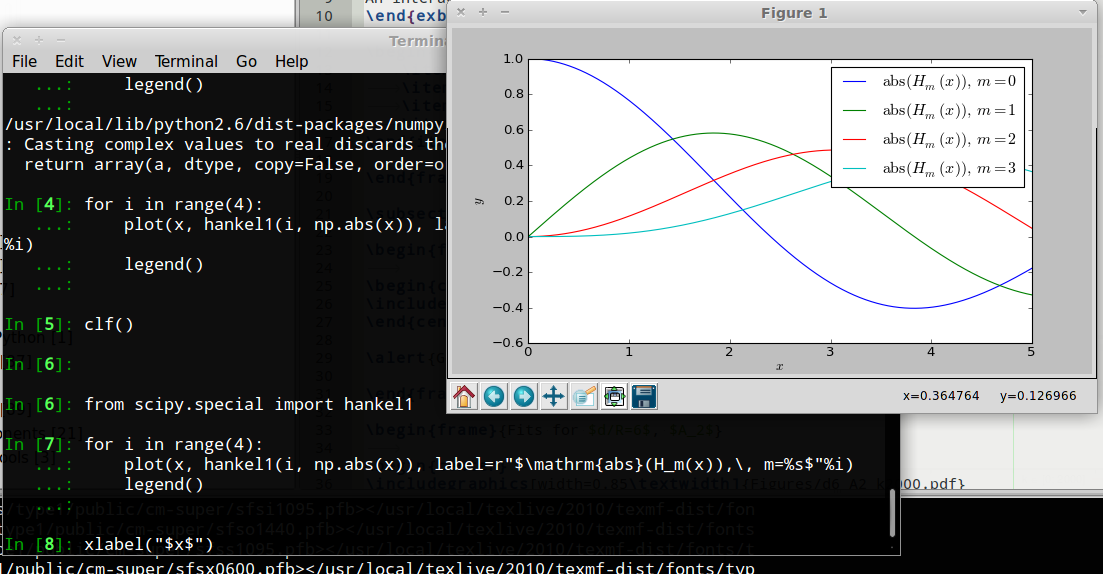
\includegraphics[width=\textwidth]{Figures/Ipython1.png}

\end{columns}

\end{frame}

\subsection{NumPy}

\begin{frame}{NumPy: Python meets an array data type}

\begin{exbox}{NumPy}
Fast and convenient array operations
\end{exbox}

\begin{itemize}
    \item Lists: + does join, not add!
    \item NumPy array: basic vector/matrix data type
    \item Convenience functions (e.g. {\texttt{linspace(), zeros(), loadtxt()...}})
    \item Array slicing
    \item element-wise operations
    \item Code using NumPy reads and writes very similar to modern Fortran
    (slicing, vector valued indices...)
\end{itemize}

\end{frame}

\begin{frame}[fragile]{NumPy by examples}

\begin{Verbatim}[commandchars=\\\{\}]
\PY{k+kn}{import} \PY{n+nn}{numpy} \PY{k+kn}{as} \PY{n+nn}{np}

\PY{n}{a} \PY{o}{=} \PY{n}{np}\PY{o}{.}\PY{n}{array}\PY{p}{(}\PY{p}{[}\PY{l+m+mf}{1.0}\PY{p}{,} \PY{l+m+mf}{2.0}\PY{p}{,} \PY{l+m+mf}{3.0}\PY{p}{,} \PY{l+m+mf}{4.0}\PY{p}{]}\PY{p}{)}
\PY{n}{b} \PY{o}{=} \PY{n}{np}\PY{o}{.}\PY{n}{array}\PY{p}{(}\PY{p}{[}\PY{l+m+mf}{4.0}\PY{p}{,} \PY{l+m+mf}{3.0}\PY{p}{,} \PY{l+m+mf}{2.0}\PY{p}{,} \PY{l+m+mf}{1.0}\PY{p}{]}\PY{p}{)}
\PY{k}{for} \PY{n}{item} \PY{o+ow}{in} \PY{n}{a}\PY{p}{:} \PY{c}{\PYZsh{} arrays are iterable}
    \PY{k}{print}\PY{p}{(}\PY{n}{item}\PY{p}{)}
\PY{n}{c} \PY{o}{=} \PY{n}{a} \PY{o}{+} \PY{n}{b} \PY{c}{\PYZsh{} c = [5, 5, 5, 5]}
\PY{k}{print}\PY{p}{(}\PY{n}{a}\PY{p}{[}\PY{l+m+mi}{0}\PY{p}{:}\PY{l+m+mi}{3}\PY{p}{:}\PY{l+m+mi}{2}\PY{p}{]}\PY{p}{)} \PY{c}{\PYZsh{} 1.0, 3.0; last element not included!}
\PY{n}{a}\PY{p}{[}\PY{l+m+mi}{0}\PY{p}{:}\PY{l+m+mi}{3}\PY{p}{]} \PY{o}{=} \PY{n}{b}\PY{p}{[}\PY{l+m+mi}{0}\PY{p}{:}\PY{o}{-}\PY{l+m+mi}{1}\PY{p}{]}

\PY{k}{print}\PY{p}{(}\PY{n}{a}\PY{o}{*}\PY{n}{b}\PY{p}{)} \PY{c}{\PYZsh{} prints [4, 6, 6, 4], not the scalar product!}
\end{Verbatim}


\end{frame}

\subsection{SciPy}

\begin{frame}{SciPy}

\begin{exbox}{SciPy}
Numerical algorithms using NumPy arrays
\end{exbox}

Wrappers around well-established libraries\\[1.0ex]

Submodules:

\begin{columns}

\column{0.5\textwidth}

\begin{itemize}
    \item {\texttt{linalg}}: linear algebra (lapack)
    \item{\texttt{sparse}}: sparse matrices
    \item {\texttt{fft}}: FFT (fftpack)
    \item {\texttt{optimize}}: optimization, zeros (minpack)
\end{itemize}


\column{0.5\textwidth}

\begin{itemize}
    \item {\texttt{integration}}: integration (quadpack, odepack)
    \item {\texttt{special}}: special functions (amos...)
    \item {\texttt{signal}}: signal processing
\end{itemize}

\end{columns}

\end{frame}

\begin{frame}[fragile]{SciPy: an example}

\begin{Verbatim}[commandchars=\\\{\}]
\PY{k+kn}{import} \PY{n+nn}{numpy} \PY{k+kn}{as} \PY{n+nn}{np}
\PY{k+kn}{from} \PY{n+nn}{scipy.optimize} \PY{k+kn}{import} \PY{n}{curve\PYZus{}fit}
\PY{k+kn}{from} \PY{n+nn}{matplotlib.pyplot} \PY{k+kn}{import} \PY{n}{plot}\PY{p}{,} \PY{n}{show}\PY{p}{,} \PY{n}{legend}

\PY{n}{x}\PY{p}{,} \PY{n}{yExp} \PY{o}{=} \PY{n}{np}\PY{o}{.}\PY{n}{loadtxt}\PY{p}{(}\PY{l+s}{"}\PY{l+s}{func.dat}\PY{l+s}{"}\PY{p}{,} \PY{n}{unpack}\PY{o}{=}\PY{n+nb+bp}{True}\PY{p}{)}
\PY{n}{plot}\PY{p}{(}\PY{n}{x}\PY{p}{,} \PY{n}{yExp}\PY{p}{,} \PY{n}{ls}\PY{o}{=}\PY{l+s}{"}\PY{l+s}{--}\PY{l+s}{"}\PY{p}{,} \PY{n}{c}\PY{o}{=}\PY{l+s}{"}\PY{l+s}{blue}\PY{l+s}{"}\PY{p}{,} \PY{n}{lw}\PY{o}{=}\PY{l+s}{"}\PY{l+s}{1.5}\PY{l+s}{"}\PY{p}{,} \PY{n}{label}\PY{o}{=}\PY{l+s}{"}\PY{l+s}{Exp.}\PY{l+s}{"}\PY{p}{)}

\PY{k}{def} \PY{n+nf}{fitFunc}\PY{p}{(}\PY{n}{x}\PY{p}{,} \PY{n}{a}\PY{p}{,} \PY{n}{b}\PY{p}{,} \PY{n}{c}\PY{p}{)}\PY{p}{:}
    \PY{k}{return} \PY{n}{a}\PY{o}{*}\PY{n}{np}\PY{o}{.}\PY{n}{exp}\PY{p}{(}\PY{o}{-}\PY{n}{b}\PY{o}{*}\PY{n}{x}\PY{p}{)} \PY{o}{+} \PY{n}{c}

\PY{n}{pOpt}\PY{p}{,} \PY{n}{pCov} \PY{o}{=} \PY{n}{curve\PYZus{}fit}\PY{p}{(}\PY{n}{fitFunc}\PY{p}{,} \PY{n}{x}\PY{p}{,} \PY{n}{yExp}\PY{p}{)}
\PY{n}{yFit} \PY{o}{=} \PY{n}{fitFunc}\PY{p}{(}\PY{n}{x}\PY{p}{,} \PY{n}{a}\PY{o}{=}\PY{n}{pOpt}\PY{p}{[}\PY{l+m+mi}{0}\PY{p}{]}\PY{p}{,} \PY{n}{b}\PY{o}{=}\PY{n}{pOpt}\PY{p}{[}\PY{l+m+mi}{1}\PY{p}{]}\PY{p}{,} \PY{n}{c}\PY{o}{=}\PY{n}{pOpt}\PY{p}{[}\PY{l+m+mi}{2}\PY{p}{]}\PY{p}{)}
\PY{n}{plot}\PY{p}{(}\PY{n}{x}\PY{p}{,} \PY{n}{yFit}\PY{p}{,} \PY{n}{label}\PY{o}{=}\PY{l+s}{"}\PY{l+s}{Fit: \PYZdl{}a = }\PY{l+s+si}{\PYZpc{}s}\PY{l+s}{; b = }\PY{l+s+si}{\PYZpc{}s}\PY{l+s}{; c= }\PY{l+s+si}{\PYZpc{}s}\PY{l+s}{\PYZdl{}}\PY{l+s}{"}\PYZbs{}
     \PY{o}{\PYZpc{}}\PY{p}{(}\PY{n}{pOpt}\PY{p}{[}\PY{l+m+mi}{0}\PY{p}{]}\PY{p}{,} \PY{n}{pOpt}\PY{p}{[}\PY{l+m+mi}{1}\PY{p}{]}\PY{p}{,} \PY{n}{pOpt}\PY{p}{[}\PY{l+m+mi}{2}\PY{p}{]}\PY{p}{)}\PY{p}{,} \PY{n}{ls}\PY{o}{=}\PY{l+s}{"}\PY{l+s}{-}\PY{l+s}{"}\PY{p}{,} \PY{n}{lw}\PY{o}{=}\PY{l+s}{"}\PY{l+s}{1.5}\PY{l+s}{"}\PY{p}{,} \PY{n}{c}\PY{o}{=}\PY{l+s}{"}\PY{l+s}{r}\PY{l+s}{"}\PY{p}{)}
\PY{n}{legend}\PY{p}{(}\PY{p}{)}\PY{p}{;} \PY{n}{show}\PY{p}{(}\PY{p}{)}
\end{Verbatim}


\end{frame}

\begin{frame}{SciPy: the example's output}

\begin{center}
    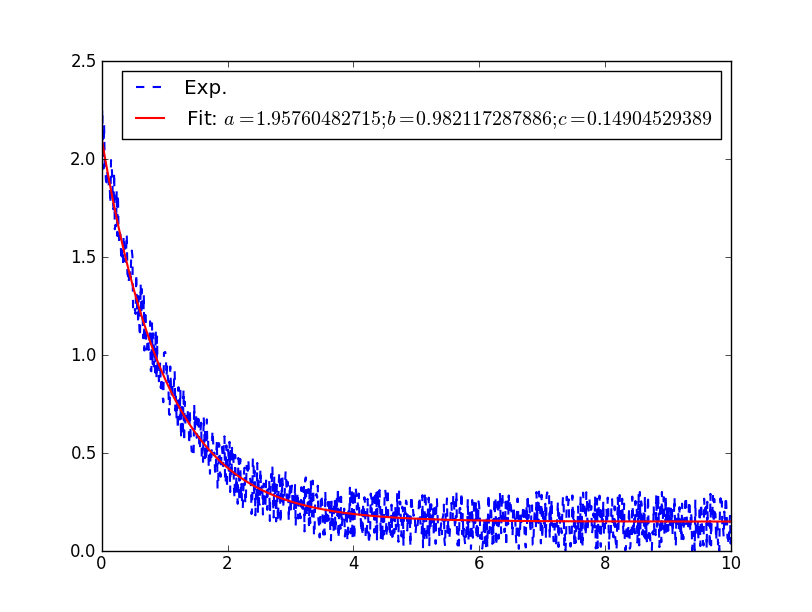
\includegraphics[width=0.8\textwidth]{Figures/fit-png}
\end{center}

Already used here: \emph{Matplotlib}

\end{frame}

\subsection{Matplotlib}

\begin{frame}{Matplotlib}

(mostly) 2D plots

\begin{center}
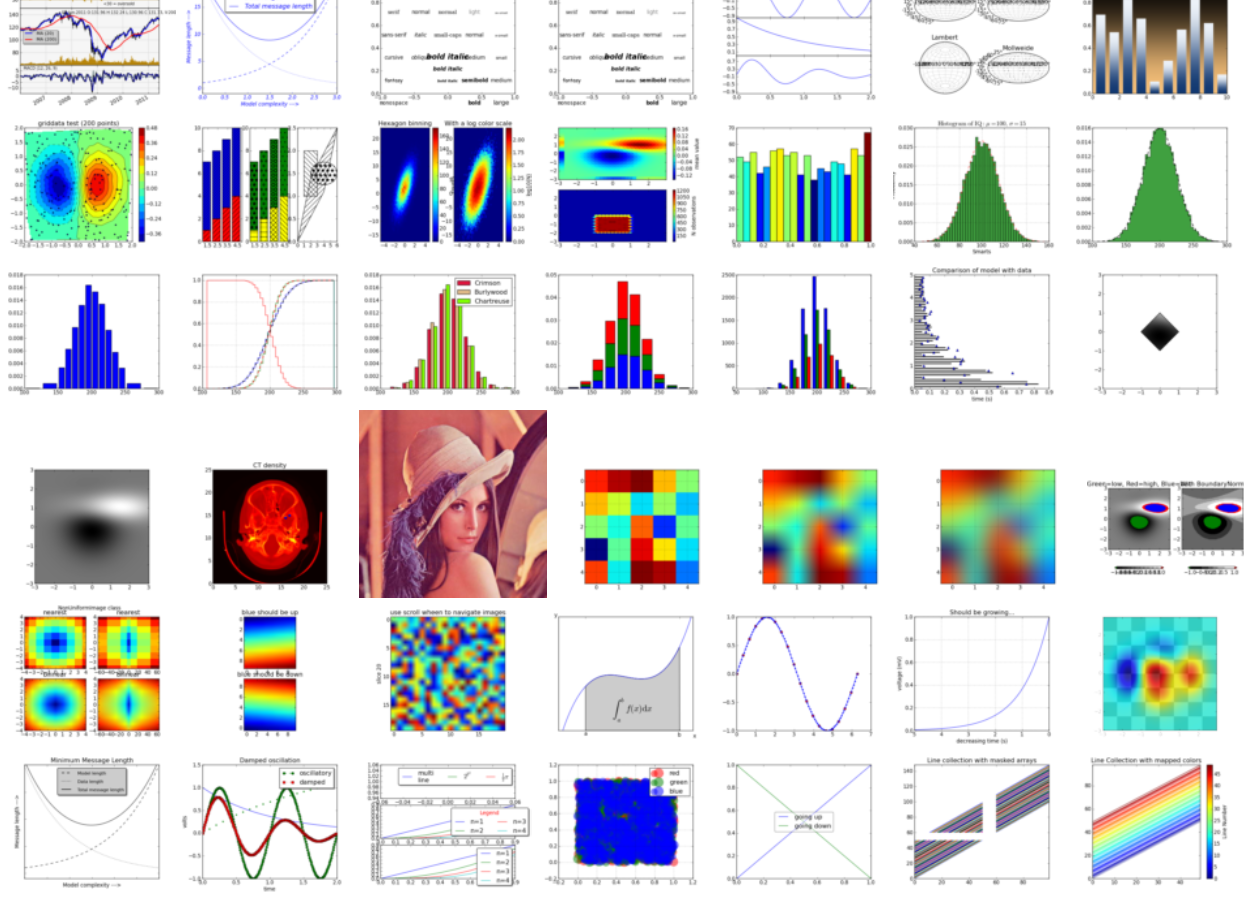
\includegraphics[width=0.8\textwidth]{Figures/mpl}
\end{center}

Pylab: MatLab alternative for interactive work
\end{frame}


\begin{frame}{Some Pylab: the logistic map $x_{n+1}= rx_n(1-x_n)$}
\input{Pygsnippets/logMap.tex}
\end{frame}

\begin{frame}{Some Pylab: the logistic map $x_{n+1}= rx_n(1-x_n)$}

The last script produces this image:

\begin{center}
    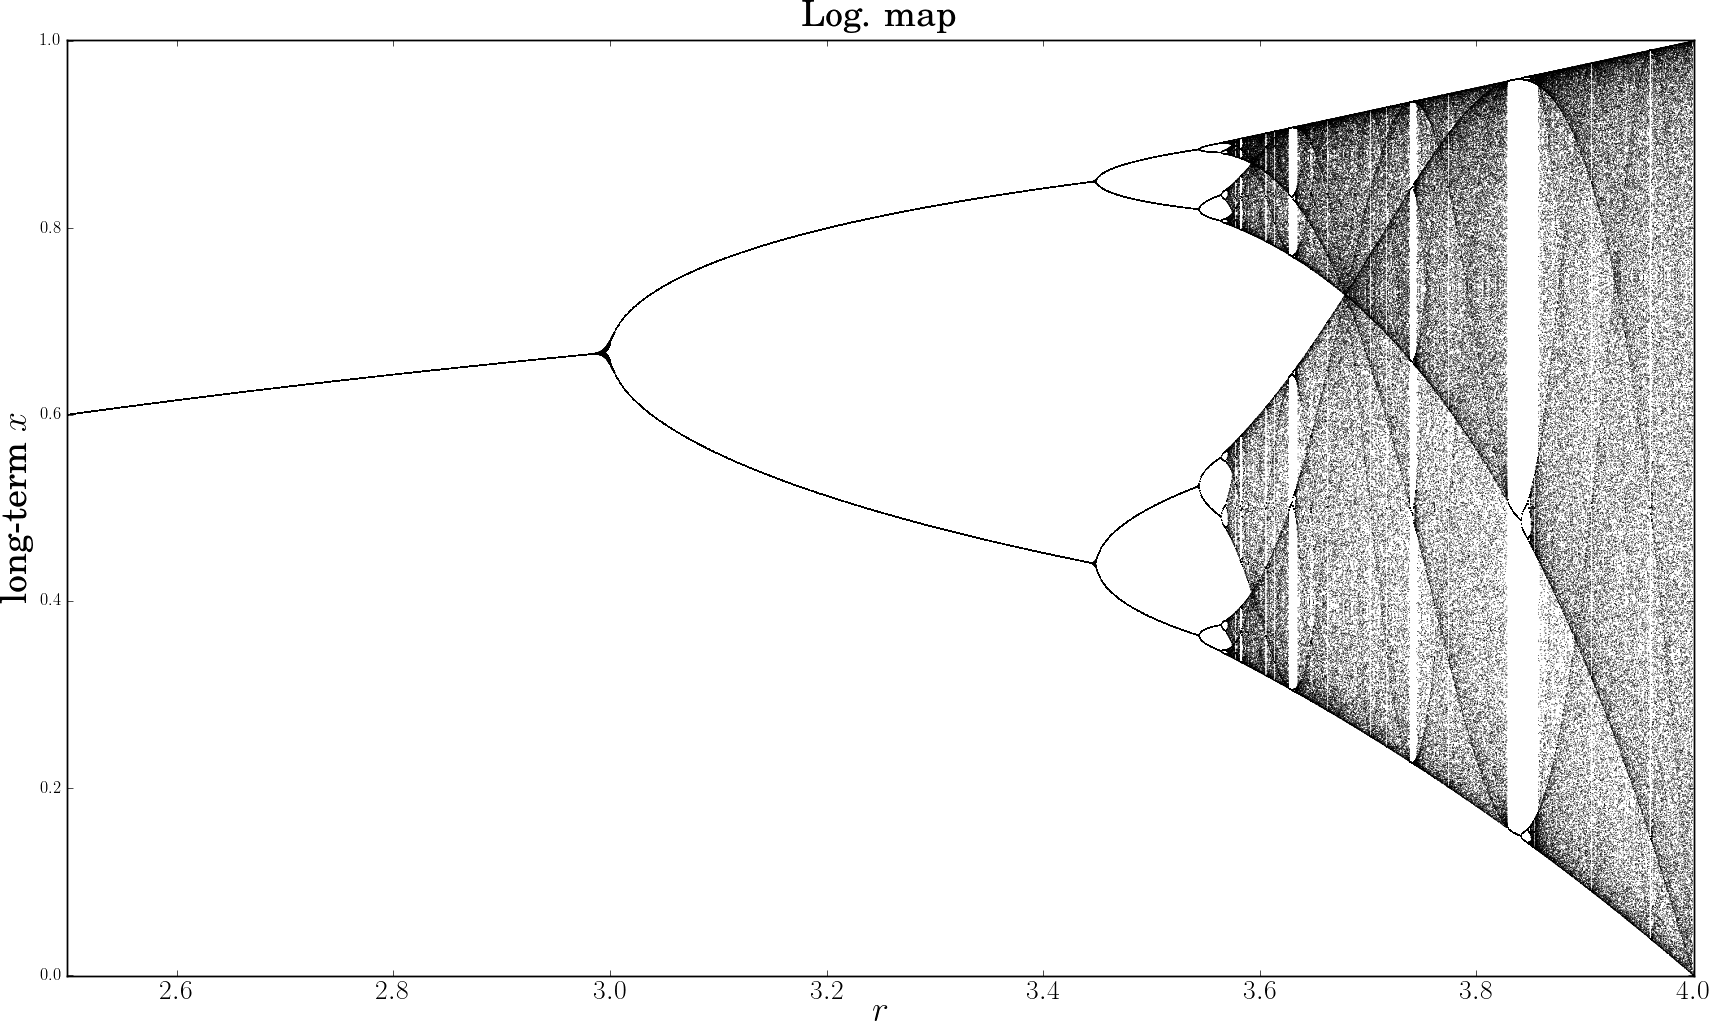
\includegraphics[width=0.9\textwidth]{Figures/logMap}
\end{center}

\end{frame}

\section{Faster Python and Glueing}

\subsection{Python as a glue}

\begin{frame}{Using Python as glue}

Python can wrap different different other programming languages\\[1ex]

\begin{exbox}{{\texttt{Cython}}}
    compiled, \emph{typed} Python - interface C/C++ code
\end{exbox}

\begin{exbox}{{\texttt{f2py}}}
    Fortran wrapper, included in NumPy
\end{exbox}

Why do that?
\begin{columns}
    
\column{0.5\textwidth}
\begin{itemize}
    \item Python can be \emph{slow}
    \item Python loops are slow
    \item calling Python functions is slow
\end{itemize}

\column{0.5\textwidth}
\begin{itemize}
    \item Wrap external C/Fortran... libraries
    \item Happily/unfortunately (?) there is legacy code
\end{itemize}

\end{columns}

\end{frame}

\subsection{A Problem}

\begin{frame}[fragile]{Problem: $\mathrm{sinc}(x)^{2}$}

\begin{Verbatim}[commandchars=\\\{\}]
\PY{k+kn}{import} \PY{n+nn}{numpy} \PY{k+kn}{as} \PY{n+nn}{np}
\PY{k+kn}{from} \PY{n+nn}{math} \PY{k+kn}{import} \PY{n}{sin}\PY{p}{,} \PY{n}{pi}

\PY{k}{def} \PY{n+nf}{sincSquare}\PY{p}{(}\PY{n}{x}\PY{p}{)}\PY{p}{:}
    \PY{l+s+sd}{"""Return the sinc(x) = (sin(x)/x)**2 of the array}
\PY{l+s+sd}{    argument x.}
\PY{l+s+sd}{    """}
    \PY{n}{retVal} \PY{o}{=} \PY{n}{np}\PY{o}{.}\PY{n}{zeros\PYZus{}like}\PY{p}{(}\PY{n}{x}\PY{p}{)}
    \PY{k}{for} \PY{n}{i} \PY{o+ow}{in} \PY{n+nb}{range}\PY{p}{(}\PY{n+nb}{len}\PY{p}{(}\PY{n}{x}\PY{p}{)}\PY{p}{)}\PY{p}{:}
        \PY{n}{retVal}\PY{p}{[}\PY{n}{i}\PY{p}{]} \PY{o}{=} \PY{p}{(}\PY{n}{sin}\PY{p}{(}\PY{n}{pi}\PY{o}{*}\PY{n}{x}\PY{p}{[}\PY{n}{i}\PY{p}{]}\PY{p}{)} \PY{o}{/} \PY{p}{(}\PY{n}{pi}\PY{o}{*}\PY{n}{x}\PY{p}{[}\PY{n}{i}\PY{p}{]}\PY{p}{)}\PY{p}{)}\PY{o}{*}\PY{o}{*}\PY{l+m+mi}{2}

    \PY{k}{return} \PY{n}{retVal}
\end{Verbatim}


\pause
$10^{6}$ array elements: {\texttt{1 loops, best of 3: 4.91 s per loop}}
\end{frame}


\begin{frame}{First attempt: use NumPy array operations}

\begin{Verbatim}[commandchars=\\\{\}]
\PY{k+kn}{import} \PY{n+nn}{numpy} \PY{k+kn}{as} \PY{n+nn}{np}

\PY{k}{def} \PY{n+nf}{sincSquareNumPy1}\PY{p}{(}\PY{n}{x}\PY{p}{)}\PY{p}{:}

    \PY{k}{return} \PY{p}{(}\PY{n}{np}\PY{o}{.}\PY{n}{sin}\PY{p}{(}\PY{n}{np}\PY{o}{.}\PY{n}{pi}\PY{o}{*}\PY{n}{x}\PY{p}{[}\PY{p}{:}\PY{p}{]}\PY{p}{)}\PY{o}{/}\PY{p}{(}\PY{n}{np}\PY{o}{.}\PY{n}{pi}\PY{o}{*}\PY{n}{x}\PY{p}{[}\PY{p}{:}\PY{p}{]}\PY{p}{)}\PY{p}{)}\PY{o}{*}\PY{o}{*}\PY{l+m+mi}{2}

\PY{k}{def} \PY{n+nf}{sincSquareNumPy2}\PY{p}{(}\PY{n}{x}\PY{p}{)}\PY{p}{:}

    \PY{k}{return} \PY{n}{np}\PY{o}{.}\PY{n}{sinc}\PY{p}{(}\PY{n}{x}\PY{p}{[}\PY{p}{:}\PY{p}{]}\PY{p}{)}\PY{o}{*}\PY{o}{*}\PY{l+m+mi}{2}
\end{Verbatim}


\pause
$10^{6}$ array elements: first function: {\texttt{10 loops, best of 3: 73 ms per loop}},
second function: {\texttt{10 loops, best of 3: 92.9 ms per loop}}4

\end{frame}

\subsection{Cython by example}

\begin{frame}{How Cython works}

\begin{exbox}{Cython}
compiled, possibly typed Python:\\[1ex]
{\texttt{.pyx file}} $\stackrel{\text{Cython}}{\Longrightarrow}$ {\texttt{.c file}} $\stackrel{\text{C compiler}}{\Longrightarrow}$ {\texttt{.so/.dll file}}
\end{exbox}

\begin{itemize}
    \item various levels of typing possible
    \item C output and Cython's opinion on code speed can easily be
    inspected (optional {\texttt{.html}} output)
    \item interface C libraries
\end{itemize}

\end{frame}

\begin{frame}[fragile]{$\mathrm{sinc}(x)^{2}$ - Cython, Version 1}

\begin{Verbatim}[commandchars=\\\{\}]
\PY{k}{cdef} \PY{k+kr}{extern} \PY{k}{from} \PY{l+s}{"}\PY{l+s}{math.h}\PY{l+s}{"}\PY{p}{:}
    \PY{n}{double} \PY{n}{sin}\PY{p}{(}\PY{n}{double}\PY{p}{)}
    \PY{n}{double} \PY{n+nb}{pow}\PY{p}{(}\PY{n}{double}\PY{p}{,} \PY{n+nb}{int}\PY{p}{)}

\PY{k}{def} \PY{n+nf}{sincSquareCython1}\PY{p}{(}\PY{n}{x}\PY{p}{)}\PY{p}{:}

    \PY{n}{pi} \PY{o}{=} \PY{l+m+mf}{3.1415926535897932384626433}
    \PY{n}{retVal} \PY{o}{=} \PY{n}{np}\PY{o}{.}\PY{n}{zeros\PYZus{}like}\PY{p}{(}\PY{n}{x}\PY{p}{)}

    \PY{k}{for} \PY{n}{i} \PY{o+ow}{in} \PY{n+nb}{range}\PY{p}{(}\PY{n+nb}{len}\PY{p}{(}\PY{n}{x}\PY{p}{)}\PY{p}{)}\PY{p}{:}
        \PY{n}{retVal}\PY{p}{[}\PY{n}{i}\PY{p}{]} \PY{o}{=} \PY{p}{(}\PY{n}{sin}\PY{p}{(}\PY{n}{pi}\PY{o}{*}\PY{n}{x}\PY{p}{[}\PY{n}{i}\PY{p}{]}\PY{p}{)} \PY{o}{/} \PY{p}{(}\PY{n}{pi}\PY{o}{*}\PY{n}{x}\PY{p}{[}\PY{n}{i}\PY{p}{]}\PY{p}{)}\PY{p}{)}\PY{o}{*}\PY{o}{*}\PY{l+m+mf}{2}

    \PY{k}{return} \PY{n}{retVal}
\end{Verbatim}


\pause
$10^{6}$ array elements: {\texttt{1 loops, best of 3: 4.39 s per loop}}
\end{frame}

\begin{frame}[fragile]{$\mathrm{sinc}(x)^{2}$ - Cython, Version 2}

\begin{Verbatim}[commandchars=\\\{\}]
\PY{k}{cimport} \PY{n+nn}{numpy} \PY{k}{as} \PY{n+nn}{np} \PY{c}{\PYZsh{} also C-import types}

\PY{k}{cpdef} \PY{k+kt}{np}.\PY{k+kt}{ndarray}[\PY{k+kt}{double}] \PY{k+kt}{sincSquareCython2}\PYZbs{}
    \PY{p}{(}\PY{n}{np}\PY{o}{.}\PY{n}{ndarray}\PY{p}{[}\PY{n}{double}\PY{p}{]} \PY{n}{x}\PY{p}{)}\PY{p}{:}

    \PY{k}{cdef} \PY{k+kt}{int} \PY{n+nf}{i}
    \PY{k}{cdef} \PY{k+kt}{double} \PY{n+nf}{pi} \PY{o}{=} \PY{l+m+mf}{3.1415926535897932384626433}
    \PY{k}{cdef} \PY{k+kt}{np}.\PY{k+kt}{ndarray}[\PY{k+kt}{double}] \PY{n+nf}{retVal} \PY{o}{=} \PY{n}{np}\PY{o}{.}\PY{n}{zeros\PYZus{}like}\PY{p}{(}\PY{n}{x}\PY{p}{)}

    \PY{k}{for} \PY{n}{i} \PY{o+ow}{in} \PY{n+nb}{range}\PY{p}{(}\PY{n+nb}{len}\PY{p}{(}\PY{n}{x}\PY{p}{)}\PY{p}{)}\PY{p}{:}
        \PY{n}{retVal}\PY{p}{[}\PY{n}{i}\PY{p}{]} \PY{o}{=} \PY{n+nb}{pow}\PY{p}{(}\PY{n}{sin}\PY{p}{(}\PY{n}{pi}\PY{o}{*}\PY{n}{x}\PY{p}{[}\PY{n}{i}\PY{p}{]}\PY{p}{)} \PY{o}{/} \PY{p}{(}\PY{n}{pi}\PY{o}{*}\PY{n}{x}\PY{p}{[}\PY{n}{i}\PY{p}{]}\PY{p}{)}\PY{p}{,} \PY{l+m+mf}{2}\PY{p}{)}
\end{Verbatim}


\pause
$10^{6}$ array elements: {\texttt{10 loops, best of 3: 49.1 ms per loop}}\\[0.5ex]
That's a \alert{speedup by a factor $\approx 100$}!
\end{frame}

\subsection{f2py by example}

\begin{frame}{How f2py works}

\begin{exbox}{f2py}
wrap Fortran code in Python:\\[1ex]
{\texttt{.f/.f90 file}} $\stackrel{\text{f2py}}{\Longrightarrow}$ {\texttt{.so/.dll file}}
\end{exbox}

\begin{itemize}
    \item f2py is included in NumPy
    \item exposes NumPy arrays to Fortran code
    \item once 'Fortran space' is entered, you run at full Fortran speed
\end{itemize}

\end{frame}

\begin{frame}[fragile]{$\mathrm{sinc}(x)^{2}$ - f2py, Version 1}

\begin{Verbatim}[commandchars=\\\{\}]
\PY{k}{subroutine }\PY{n+nv}{sincsquaref2py1}\PY{p}{(}\PY{n+nv}{x}\PY{p}{,} \PY{n+nv}{n}\PY{p}{,} \PY{n+nv}{outVal}\PY{p}{)}
    \PY{k}{implicit }\PY{k}{none}

\PY{k}{    }\PY{k+kt}{double precision}\PY{p}{,} \PY{k}{dimension}\PY{p}{(}\PY{n+nv}{n}\PY{p}{)}\PY{p}{,} \PY{k}{intent}\PY{p}{(}\PY{n+nv}{in}\PY{p}{)} \PY{k+kd}{::} \PY{n+nv}{x}
    \PY{k+kt}{integer}\PY{p}{,} \PY{k}{intent}\PY{p}{(}\PY{n+nv}{in}\PY{p}{)} \PY{k+kd}{::} \PY{n+nv}{n}
    \PY{k+kt}{double precision}\PY{p}{,} \PY{k}{dimension}\PY{p}{(}\PY{n+nv}{n}\PY{p}{)}\PY{p}{,} \PY{k}{intent}\PY{p}{(}\PY{n+nv}{out}\PY{p}{)} \PY{k+kd}{::} \PY{n+nv}{outVal}
    \PY{k+kt}{double precision}\PY{p}{,} \PY{k}{parameter} \PY{k+kd}{::} \PY{n+nv}{pi} \PY{o}{=} \PY{l+m+mf}{4.0}\PY{n+nv}{d0} \PY{o}{*} \PY{n+nb}{atan}\PY{p}{(}\PY{l+m+mf}{1.0}\PY{n+nv}{d0}\PY{p}{)}

    \PY{n+nv}{outVal}\PY{p}{(}\PY{p}{:}\PY{p}{)} \PY{o}{=} \PY{p}{(}\PY{n+nb}{sin}\PY{p}{(}\PY{n+nv}{pi}\PY{o}{*}\PY{n+nv}{x}\PY{p}{(}\PY{p}{:}\PY{p}{)}\PY{p}{)} \PY{o}{/} \PY{p}{(}\PY{n+nv}{pi}\PY{o}{*}\PY{n+nv}{x}\PY{p}{(}\PY{p}{:}\PY{p}{)}\PY{p}{)}\PY{p}{)}\PY{o}{**}\PY{l+m+mi}{2}

\PY{k}{end }\PY{k}{subroutine }\PY{n+nv}{sincsquaref2py1}
\end{Verbatim}


\pause
$10^{6}$ array elements: {\texttt{10 loops, best of 3: 47.4 ms per loop}}\\
Again, a \alert{speedup by a factor of $\approx 100$}!

\end{frame}

\begin{frame}[fragile]{Cheating: $\mathrm{sinc}(x)^{2}$ - f2py, Version 2 - OpenMP}

\begin{Verbatim}[commandchars=\\\{\}]
\PY{k}{subroutine }\PY{n+nv}{sincsquaref2py2}\PY{p}{(}\PY{n+nv}{x}\PY{p}{,} \PY{n+nv}{n}\PY{p}{,} \PY{n+nv}{outVal}\PY{p}{)}
    \PY{k}{implicit }\PY{k}{none}
\PY{k}{    }\PY{k+kt}{double precision}\PY{p}{,} \PY{k}{dimension}\PY{p}{(}\PY{n+nv}{n}\PY{p}{)}\PY{p}{,} \PY{k}{intent}\PY{p}{(}\PY{n+nv}{in}\PY{p}{)} \PY{k+kd}{::} \PY{n+nv}{x}
    \PY{k+kt}{integer}\PY{p}{,} \PY{k}{intent}\PY{p}{(}\PY{n+nv}{in}\PY{p}{)} \PY{k+kd}{::} \PY{n+nv}{n}
    \PY{k+kt}{double precision}\PY{p}{,} \PY{k}{dimension}\PY{p}{(}\PY{n+nv}{n}\PY{p}{)}\PY{p}{,} \PY{k}{intent}\PY{p}{(}\PY{n+nv}{out}\PY{p}{)} \PY{k+kd}{::} \PY{n+nv}{outVal}
    \PY{k+kt}{integer} \PY{k+kd}{::} \PY{n+nv}{i}
    \PY{k+kt}{double precision}\PY{p}{,} \PY{k}{parameter} \PY{k+kd}{::} \PY{n+nv}{pi} \PY{o}{=} \PY{l+m+mf}{4.0}\PY{n+nv}{d0} \PY{o}{*} \PY{n+nb}{atan}\PY{p}{(}\PY{l+m+mf}{1.0}\PY{n+nv}{d0}\PY{p}{)}
    \PY{c}{!\PYZdl{}OMP PARALLEL DO SHARED(x, outVal)}
    \PY{k}{do }\PY{n+nv}{i} \PY{o}{=} \PY{l+m+mi}{1}\PY{p}{,} \PY{n+nv}{n}
        \PY{n+nv}{outVal}\PY{p}{(}\PY{n+nv}{i}\PY{p}{)} \PY{o}{=} \PY{p}{(}\PY{n+nb}{sin}\PY{p}{(}\PY{n+nv}{pi}\PY{o}{*}\PY{n+nv}{x}\PY{p}{(}\PY{n+nv}{i}\PY{p}{)}\PY{p}{)} \PY{o}{/} \PY{p}{(}\PY{n+nv}{pi}\PY{o}{*}\PY{n+nv}{x}\PY{p}{(}\PY{n+nv}{i}\PY{p}{)}\PY{p}{)}\PY{p}{)}\PY{o}{**}\PY{l+m+mi}{2}
    \PY{k}{end }\PY{k}{do}
    \PY{c}{!\PYZdl{}OMP END PARALLEL DO}
\PY{k}{end }\PY{k}{subroutine }\PY{n+nv}{sincsquaref2py2}
\end{Verbatim}


\pause
$10^{6}$ array elements, 2 Threads: {\texttt{10 loops, best of 3: 33.5 ms per loop}}
\end{frame}

\begin{frame}{$\mathrm{sinc}(x)^{2}$ - Overview}

Benchmark for an Intel i7:

\begin{center}
    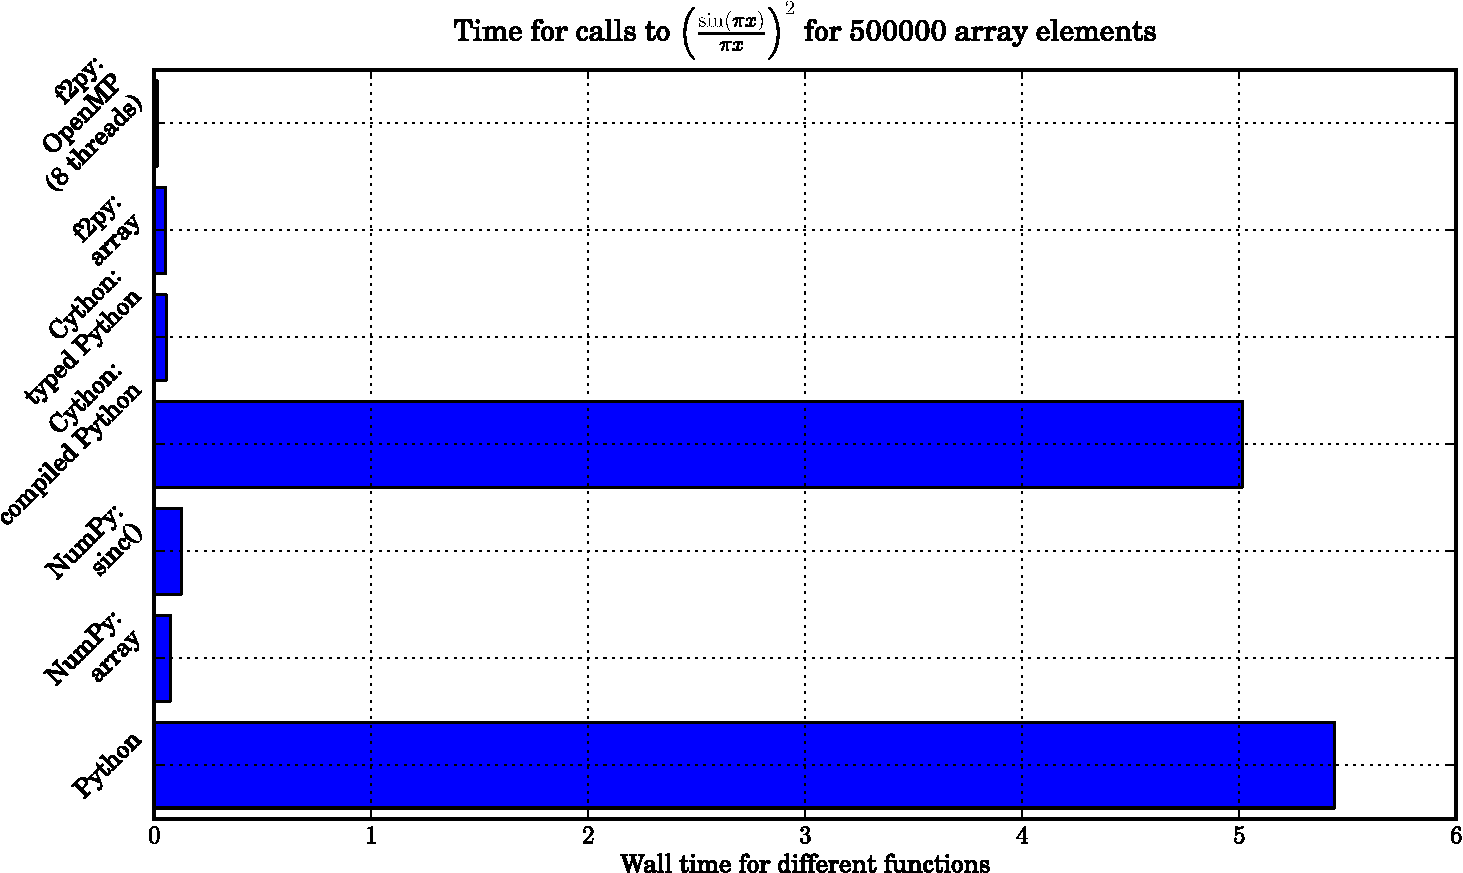
\includegraphics[width=1.0\textwidth]{Figures/benchmark}
\end{center}

Comparison: pure Fortran: 

\end{frame}

\subsection{Techniques for faster Scripts}

\begin{frame}{Techniques for faster Scripts}

After you have written a prototype in Python with NumPy and SciPy,
check if your code is already fast enough. If not,

\begin{itemize}
    \item profile your script (IPython's {\texttt{run -p}} or
    {\texttt{cProfile}} module...) to find bottlenecks
    \item if a large numbers of function calls is the bottleneck,
    typing and using  Cython's {\texttt{cdef/cpdef}} for C calling
    conventions speeds your code up at the cost of flexibility
    \item loops greatly benefit from typing, too
    \item consider moving heavy computations to Fortran/C completely -
    f2py and Cython will help you wrapping
\end{itemize}

\end{frame}

\subsection{MPI in Python}

\begin{frame}{Slightly OffTopic: mpi4py}

\begin{exbox}{mpi4py}
    Interface MPI in Python
\end{exbox}

\begin{itemize}
    \item speed-up pure Python by parallelization using MPI (OpenMPI, mpich...)
    \item mpi4py also works with f2py and Cython (?)
    \item[$\rightarrow$] run the steering Python script with
    {\texttt{mpirun...}}, take care of the communicator there and use
    it in Fortran, too
\end{itemize}

Alternatives:

\begin{itemize}
    \item IPython's parallel computing facilities
\end{itemize}

\end{frame}

\begin{frame}[fragile]{Slightly OffTopic: mpi4py}

\begin{Verbatim}[commandchars=\\\{\}]
\PY{k+kn}{from} \PY{n+nn}{mpi4py} \PY{k+kn}{import} \PY{n}{MPI}

\PY{n}{MPIroot} \PY{o}{=} \PY{l+m+mi}{0} \PY{c}{\PYZsh{} define the root process}
\PY{n}{MPIcomm} \PY{o}{=} \PY{n}{MPI}\PY{o}{.}\PY{n}{COMM\PYZus{}WORLD} \PY{c}{\PYZsh{} MPI communicator}

\PY{n}{MPIrank}\PY{p}{,} \PY{n}{MPIsize} \PY{o}{=} \PY{n}{MPIcomm}\PY{o}{.}\PY{n}{Get\PYZus{}rank}\PY{p}{(}\PY{p}{)}\PY{p}{,} \PY{n}{MPIcomm}\PY{o}{.}\PY{n}{Get\PYZus{}size}\PY{p}{(}\PY{p}{)}

\PY{o}{.}\PY{o}{.}\PY{o}{.}

\PY{n}{MPIcomm}\PY{o}{.}\PY{n}{Reduce}\PY{p}{(}\PY{n}{tempVals}\PY{p}{,} \PY{n}{retVal}\PY{p}{,} \PY{n}{op}\PY{o}{=}\PY{n}{MPI}\PY{o}{.}\PY{n}{SUM}\PY{p}{,} \PY{n}{root}\PY{o}{=}\PY{n}{MPIroot}\PY{p}{)}
\end{Verbatim}


\end{frame}


\section{Summary}

\subsection{Summary}

\begin{frame}{Summary}

We have...

\begin{itemize}
	\item introduced basic Python scripting
	\item shown some basic modules for scientific computing
	\item demonstrated how to wrap other languages
	\item learned how to speed Python up
\end{itemize}

\begin{alertbbox}{Take home message}
Python is a very valuable tool for Physicists
\end{alertbbox}

Slides, \LaTeX~and Python Sources available at\\
\url{http://github.com/aeberspaecher}

\end{frame}


\end{document}
